\section{Physikalische Grundlagen}
\subsection{Grundkonzept eines PET-Scanners}
	Die \textbf{Positronen-Emissions-Tomographie} ist ein bildgebendes Verfahren zur in vivo-Bechreibung von biochemischen und physiologischen Prozessen. Sie ist dadurch ein Beispiel für ein \textbf{funktionelles} Bildgebungsverfahren, das dazu dient, um Stoffwechselprozesse und Blutflüsse im menschlichen Körper zu überwachen, ohne dabei chirurgische Maßnahmen in Erwägung ziehen zu müssen. Dem Patientien wird dabei ein $\beta^+$-Strahler (ein sogenannter \textbf{Tracer}) mit einer Halbwertszeit in der Dimension von mehreren Minuten bis Stunden, welcher den physiologischen Vorgang im Körper begleitet und sich in bestimmten Strukturen anreichert. Die Tracer haben einen Protonenüberschuss, wodurch in Atomkernen der Tranceratome folgende Kernreaktion stattfindet: 
	\begin{equation*}
	p^+ \longrightarrow n + e^+ + \nu_e
	\end{equation*}\\
	Die entstandenen Positronen (Ruheenergie $E_0 = 511\ \unit{keV}$) annihilieren innerhalb weniger Millimeter mit Hüllenelektronen des umliegenden Gewebes zu zwei Photonen der Energie $E_{\gamma_1}$ und $E_{\gamma_2}$ :\\
	\begin{equation*}
		e^+ e^- \longrightarrow \gamma \gamma
	\end{equation*}
	Im Schwerpunktsystem des Lepton-Antilepton-Paares stehen die Impulse kollinear, wodurch der Gesamtimpuls verschwindet. Aufgrund der Viererimpulserhaltung muss auch der Impuls des entstandenen Photonenpaares verschwindet, wodurch sich in etwa ein 180° Winkel zwischen ihnen ergibt und ihre Energie unter Vernachlässigung der kinetischen Energie der einfallenden Teilchen ungefähr gleich der Summe der Ruheenergien des Elektron-Positron-Paares ist, d.h. $E_{\gamma_1} = E_{\gamma_2} \approx 511\ \unit{keV}$. Das ist auch der Energiewert, bei dem wir später der Peak des Energiespektrums erwarten. Hieraus können wir ein Kriterium für die Wahl eines geeigneten Tracers ableiten: Je geringer die maximale Energie des emittierten Positrons, desto geringer ist die Entfernung des Annihilationsort vom Emissionsort und desto geringer sind die Abweichungen des 180°-Winkels und des Energiepeaks der Photonen. Dadurch werden Fehlerquellen bei der Lokalisierung des Tracers minimiert.\\
	
	\minipanf
		\begin{center}
			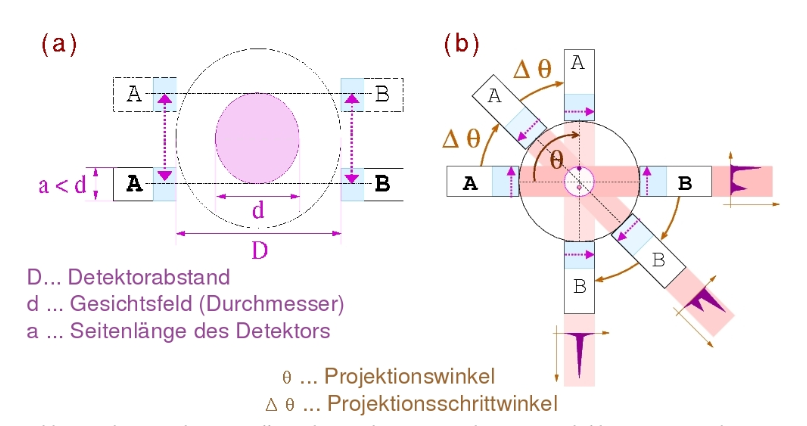
\includegraphics[width=0.8\textwidth, height=0.3\textheight]{pic/PET-Prinzip.png}
			\label{PET-Prinzip}
			\captionof{figure}{Funktionsprinzip eines PET-Scanners\cite{PA}}
		\end{center}
	\minipend 
	\hspace{3mm}
	\ \\	
	Die beiden Annihilationsphotonen der (ausgedehnten) Quellverteilung werden anschließend von zwei gegenüberliegenden Detektoren registriert. Dadurch erhalten wir die auf der Verbindungslinie integrierte (\textbf{Radon-Transformierte}) Aktivitätsverteilung, indem wir die Detektoren nun unter verschiedenen Winkeln um die Quellen rotieren. Mit Hilfe dieser Daten kann die Ausgangsverteilung über eine inverse Koordinaten-Transformation rekonstruiert werden.\cite{PA}	
	
\subsection{Koinzidenzmessungen}
	Da die gleichzeitig emittierten, also zeitlich korrelierten, Photonen in zwei verschiedenen Detektoren registriert werden, zwischen den zwei Zählsignalen aber immer eine gewisse Zeitdifferenz $\Delta t(1,2)$ existieren wird, definiert man das \textbf{Koinzidenzzeitfenster} $[\Delta t_{min}, \Delta t_{max}]$ als Intervall von Zeitdifferenzen zwischen zwei Messereignissen 1 und 2, die man noch als zeitlich korrelierte Ereignisse akzeptiert, d.h. Messereignis 1 und 2 sind (im Idealfall) zeitlich korreliert genau dann wenn: $\Delta t(1,2) \in [\Delta t_{min}, \Delta t_{max}]$. Diese Ereignisse nennt man \textbf{wahre Koinzidenzen} Die Länge des intervalls nennt man \textbf{Koinzidenzauflösungszeit}. Das Zeitintervall wird durch die Kalibrationsmessung im ersten experimentellen Teil durch Erstellen eines Histogramms von Zeitunterschieden bestimmt. Leider werden in der Praxis durch dieses Zeitfenster auch Ereignisse nachgewiesen, die physikalisch nicht korreliert sind. Diese nennt man \textbf{zufällige Koinzidenzen} und sie gilt es herauszufiltern.\cite{PA} Dies wird näher in Abschnitt (\ref{dft:kalib_mitte}) diskutiert.


\subsection{Detektoraufbau}
\subsubsection{Szintillationsdetektoren}
	Zum Nachweis der Annihilationsphotonen wird ein sogenannter \textbf{Szintillationsdetektor} verwendet. Dieser besteht aus einem geeignet präparierten anorganischen Kristall, in dem die einfallenden hochenergetischen Primärphotonen durch Wechselwirkung (Photoeffekt, Compton-Streuung und Paarbildung) mit den Hüllenelektronen angeregte Zustände erzeugen, welche beim Abregen niederenergetische Sekundärphotonen im Bereich des sichtbaren Lichts erzeugen. Dabei ist die Anzahl proportional zur Energie, die im Detektor deponiert wurde. In reinen Kristallen hat man das Problem, dass die Sekundärphotonen erneut Elektronen-Loch-Paare erzeugen können, wodurch die Photonen absorbiert werden und der Kristall somit für das entstandene Licht nicht transparent ist. Dieses Problem löst man, indem man den Kristall geeignet dotiert, d.h. man bringt Störstellen in das Gitter ein, wodurch neue Energieterme (\textbf{Aktivatorterme}) entstehen. Rekombiniert nun ein Elektron aus einem solchen Term, entsteht ein Photon, das zu langwellig ($\lambda = 300\ -\ 350\ \unit{nm}$) ist, um vom Kristall absorbiert zu werden.\\
	\minipanf
				\begin{center}
					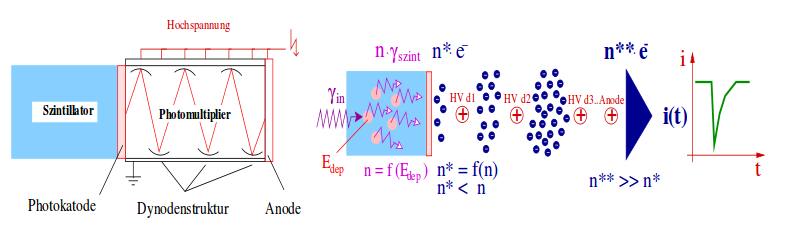
\includegraphics[width=0.8\textwidth, height=0.15\textheight]{pic/szintillator.png}
					\label{PET-Prinzip}
					\captionof{figure}{Aufbau eines Szintillationsdetektors\cite{info}}
				\end{center}
				\hspace{2mm}
	\minipend\\ 
	Diese Photonen gelangen nun zu einem \textbf{Photomultiplier}, welcher aus einer Photokathode und einer Dynodenstruktur besteht. Die Sekundärphotonen schlagen durch  Photoeffekt Elektronen aus der Kathode, welche in einem elektrischen Feld der Dynoden beschleunigt werden. Treffen diese auf eine Dynode, so werden aus dieser weitere Elektronen herausgeschlagen, wodurch die Elektronenzahl exponentiell mit der Dynodenzahl steigt. Der dadurch entstandene Stromfluss kann nun an einer Anode gemessen werden.\cite{info}

		
\subsubsection{Modifiziertes Anger-Prinzip}
	Würde man die Szintillator-Kristalle einzeln an Photomultiplier koppel, würde das örtliche Auflösungsvermögen der Messapperatur von der Größe der Multiplier begrenzt werden. Da diese aber technisch nicht beliebig klein konstruiert werden können, koppelt man mehrere Szintillatoreinheiten an einen Multiplier, indem man den Kristall durch unterschiedlich tiefe Einschnitte in eine Matrix einteilt. Im konkreten Experiment wurden 4 Photomultiplier mit einer 8x8-Szintillator-Matrix verbunden. Mit Hilfe der Einschnitte gelangen die entstehenden Sekundärphotonen über totale Reflexion auf mehrere Multiplier, an denen sie einen Stromimpuls mit einer Amplitude $A_i$ erzeugen. Die im Detektor deponierte Energie des einfallenden Photons ist dabei proportional zur Summe aus allen Stromamplituden. \\
	
	\minipanf
					\begin{center}
						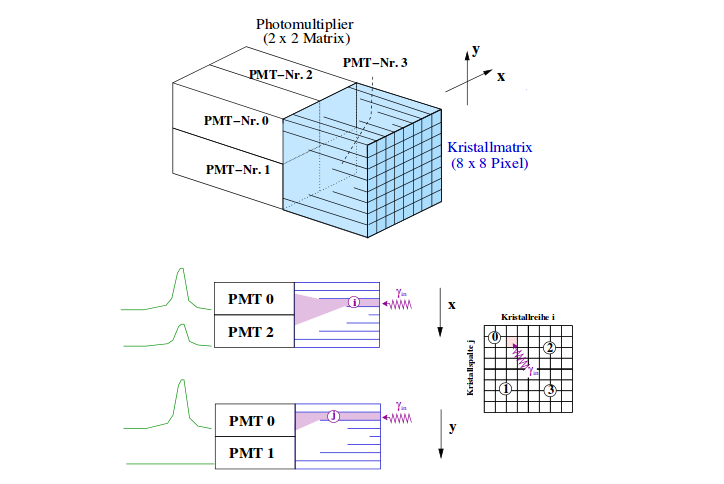
\includegraphics[width=0.8\textwidth, height=0.3\textheight]{pic/anger-prinzip.png}
						\label{PET-Prinzip}
						\captionof{figure}{Darstellung des verwendeten Blockdetektors: Vier Photomultiplier sind mit einer 8x8-Kristallmatrix aus Szintillatorkristallen verbunden\cite{info}}
					\end{center}
					\hspace{2mm}
	\minipend\\
	Der Ort des einfallenden Teilchens wird nun über Schwerpunktbildung rekonstruiert: Je 'mittiger' das Teilchen auf den Detektor trifft, desto besser werden die Sekundärephotonen auf alle vier Multiplier verteilt, wodurch in allen annähernd die gleiche Amplitude gemessen wird, d.h. es gilt: $A_0 \cong A_1 \cong A_2 \cong A_3$, was wir ohne Beschränkung der Allgemeinheit mit der Koordinate $(x = 0, y = 0)$ identifizieren. In diesem Koordinatensystem erhalten wir nun die Orte der einfallenden Teilchen:
	\begin{equation*}
	x = \frac{(A_2+A_3)-(A_0+A_1)}{\sum_{i=0}^{3} A_i}\ ;\ y = \frac{(A_0+A_2)-(A_1+A_3)}{\sum_{i=0}^{3} A_i}
	\end{equation*}